\vspace{-0.2cm}

Dataset characteristics vary substantially from BU to BU.
In our experiments, we found that data from BU1 is substantially corrected using large scale human annotation efforts to create rules for categorization which are contracted to BU1 only.
This leads to lower coverage at the expense of high precision and much lower noise, however, such kind of manual efforts are not scalable.
On the other hand, the listing feed which BU2 receives is from external data vendors who sell their feed at substantial subscription rates. 
However, the taxonomies and categorization these vendors provide are often wrong -- partly due to sellers providing wrong categories while listing as well -- see for e.g. a 15\% error reported in \cite{Shen12}.
BU2 converts taxonomies from these data vendors to their own manually and hence directly maps listings without any error correction.
We observe such instances of error in Fig. \ref{Fig:push-pull} for the leaf node ``\textit{Sneakers}'' and the listing ``\textit{1883 by Wolverine Women's Maisie Oxford Tan/Taupe Leather/Suede}'' - the correct leaf node should have been ``\textit{Other} $\rightarrow$ Women's Shoes'' (not shown in Fig. \ref{Fig:push-pull}).
Much of the problems arising in taxonomy classification of product listings has been well documented in \cite{Sun14, Shen12, Pyo16} and we do not elaborate on them unless necessary.
For BU2 dataset, the noise is distributed identically in the training and test sets and thus evaluation of the classifiers is not impeded by it.
Examples of noise in BU2 dataset, other than algorithmic taxonomy assignment problems of the data vendor, can be attributed to incomplete or over complete title text and navigational breadcrumb extractions from crawled pages in the wild.

\begin{wrapfigure}{r}{0.42\textwidth}
	\centering
	\vspace{-0.5cm}
	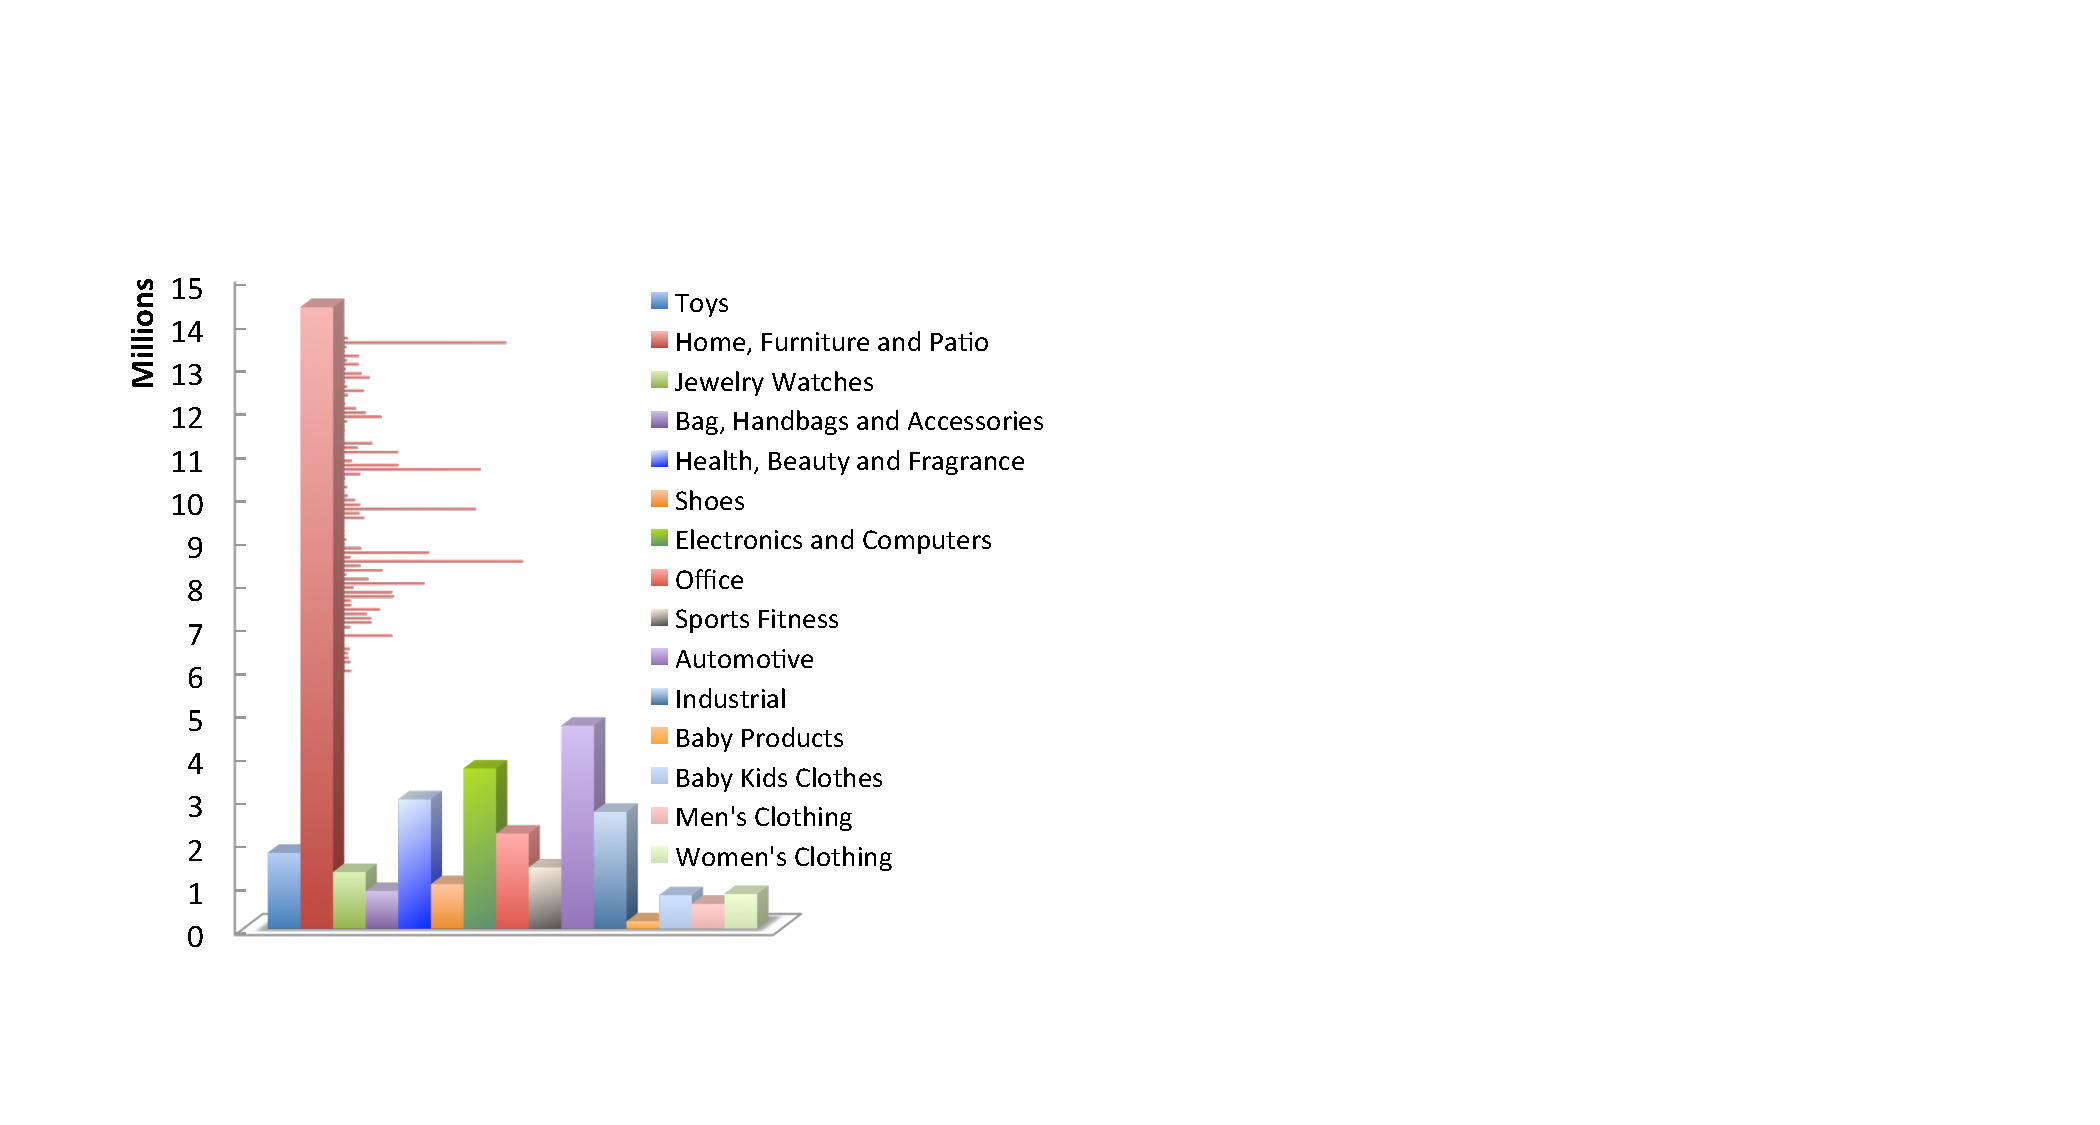
\includegraphics[width=0.42\textwidth]{images/BU2-dataset-Dec2015}
	\vspace{-0.6cm}
	\caption{{\small Dataset from BU2 -- Dec 2015 snapshot. Total number of de-duplicated listings is 40 million.}}
	\vspace{-0.5cm}
	\label{Figure_BU2-datset-earlier}
\end{wrapfigure}
The absence of a ground-truth training set from BU2 constrains us to rely on this noisy dataset for training our classifiers. 
Needless to mention, the amount of this kind of ``label flip'' error is not nominal and it is hard to correct without manual scans of millions of listings -- an impossible task which is mitigated to some extent for BU2's dataset using topic model based noise analysis (Section \ref{Subsect:BU2-noise-analysis}).
In an industrial setting, automatic categorizations are continuously eliminated manually either in-house (low budget) or through external organizations such as CrowdFlower\footnote{\scriptsize{\url{https://www.crowdflower.com/crowdflower-attacks-data-scientists-biggest-challenge-incomplete-messy-data/}}} \cite{Sun14}.
However, since manual annotation is expensive, using some proxy for ground truths as a viable alternative has also been mentioned in \cite{Shen12}.


\begin{wrapfigure}{l}{0.45\textwidth}
	\centering
	\vspace{-0.6cm}
	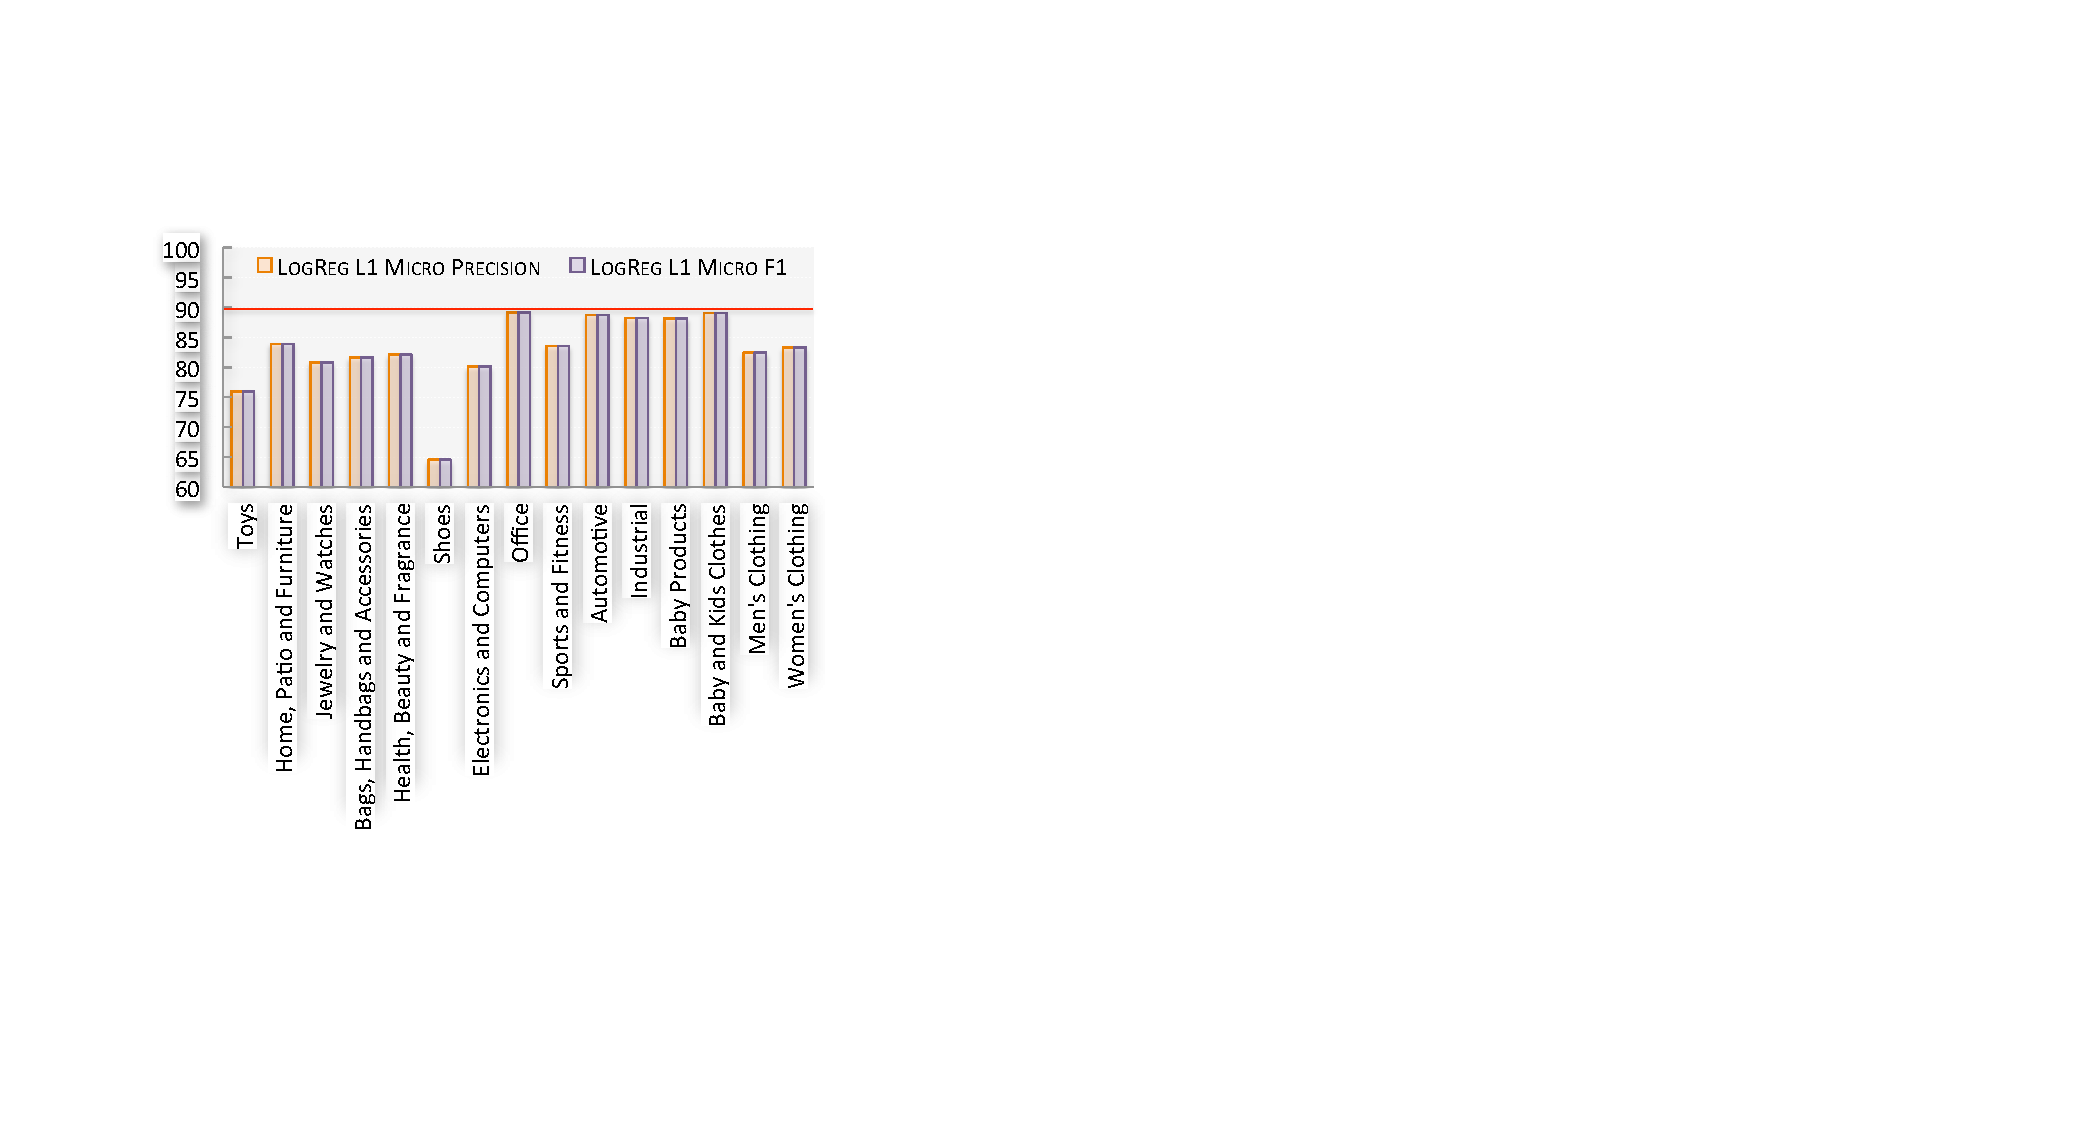
\includegraphics[width=0.45\textwidth]{images/BU2-Dec2015-LogRegL1}
	\vspace{-0.7cm}
	\caption{{\small Micro precision and micro F1 across 15 top level categories obtained using 10\% of the 40 million listings as test set for the dataset in Fig. \ref{Figure_BU2-datset-earlier}}}
	\label{Figure_BU2-WUC-LogRegL1}
	\vspace{-0.5cm}
\end{wrapfigure} 
Dataset imbalance is also a major problem in product listing datasets for building classification models.
Most loss functions that are not resistant to imbalance generalize very poorly without resorting to any subsampling techniques \cite{Chawla02:SMOTE}. 
Noting the potential pitfalls in subsampling \cite{Sun14}, we instead, resort to cross-entropy (logistic) loss functions which are more resistant to imbalance particularly with suitable regularizers (Section \ref{Sect:experimental_setup}). 
A preview of the imbalance in BU2's dataset is shown in Fig. \ref{Figure_BU2-datset-earlier} where a disproportionate number of listings appear in the ``Home, Patio and Furniture'' category.
In the experiments shown in Section \ref{Sect:results}, we use BU2's data snapshot from Feb 2016 which initially consists of 204 million \textbf{deduplicated} listings from 277 merchants, dropping down to 60 million after aggressive cleanup (Section \ref{Subsect:BU2-noise-analysis}).



Our initial experiments using the noisy data in Fig. \ref{Figure_BU2-datset-earlier} using a one vs. one logistic regression model with L1 regularization \cite{Yu13:EBay,LibShortText} show promising results (see Fig. \ref{Figure_BU2-WUC-LogRegL1}) but their method do not attain a requirement of $90\% \pm \epsilon$  \textit{mean} micro precision across the level one taxonomies.
Logistic Regression (henceforth LogReg) with L1 achieves 83\% \textit{mean} micro precision (F1 values differed only in the third decimal place) for 10\% test dataset consisting of 4 million listings.
The level one classification is a much easier problem and most classifiers achieve 90\% micro precision and F1 for all of the BU datasets considered here with Gradient Boosted Tree (henceforth GBT) \cite{Friedman:GBT} and Convolutional Neural Networks (henceforth CNN) \cite{LeBe95, Kim14} performing the best. 
Classifier performance for the listings in the branches of the ``Shoes'' subtree has been very poor and this resulted in a novel way to identify the pattern of noise in whole of BU2's dataset with unsupervised topic models and minimal manual analysis (Section \ref{Subsect:BU2-noise-analysis}).

\begin{figure}[h]
	\centering
	\vspace{-0.8cm}
	\subfloat[{{\footnotesize BU1 dataset: Total subtrees with taxonomy - 16; Total branches in all subtrees - 1146; Total listings in all subtrees - 12.61 million; Pearson correlation coeff. for branches vs. listings - 0.643 }}]{\label{Fig:BU1-branches+KL}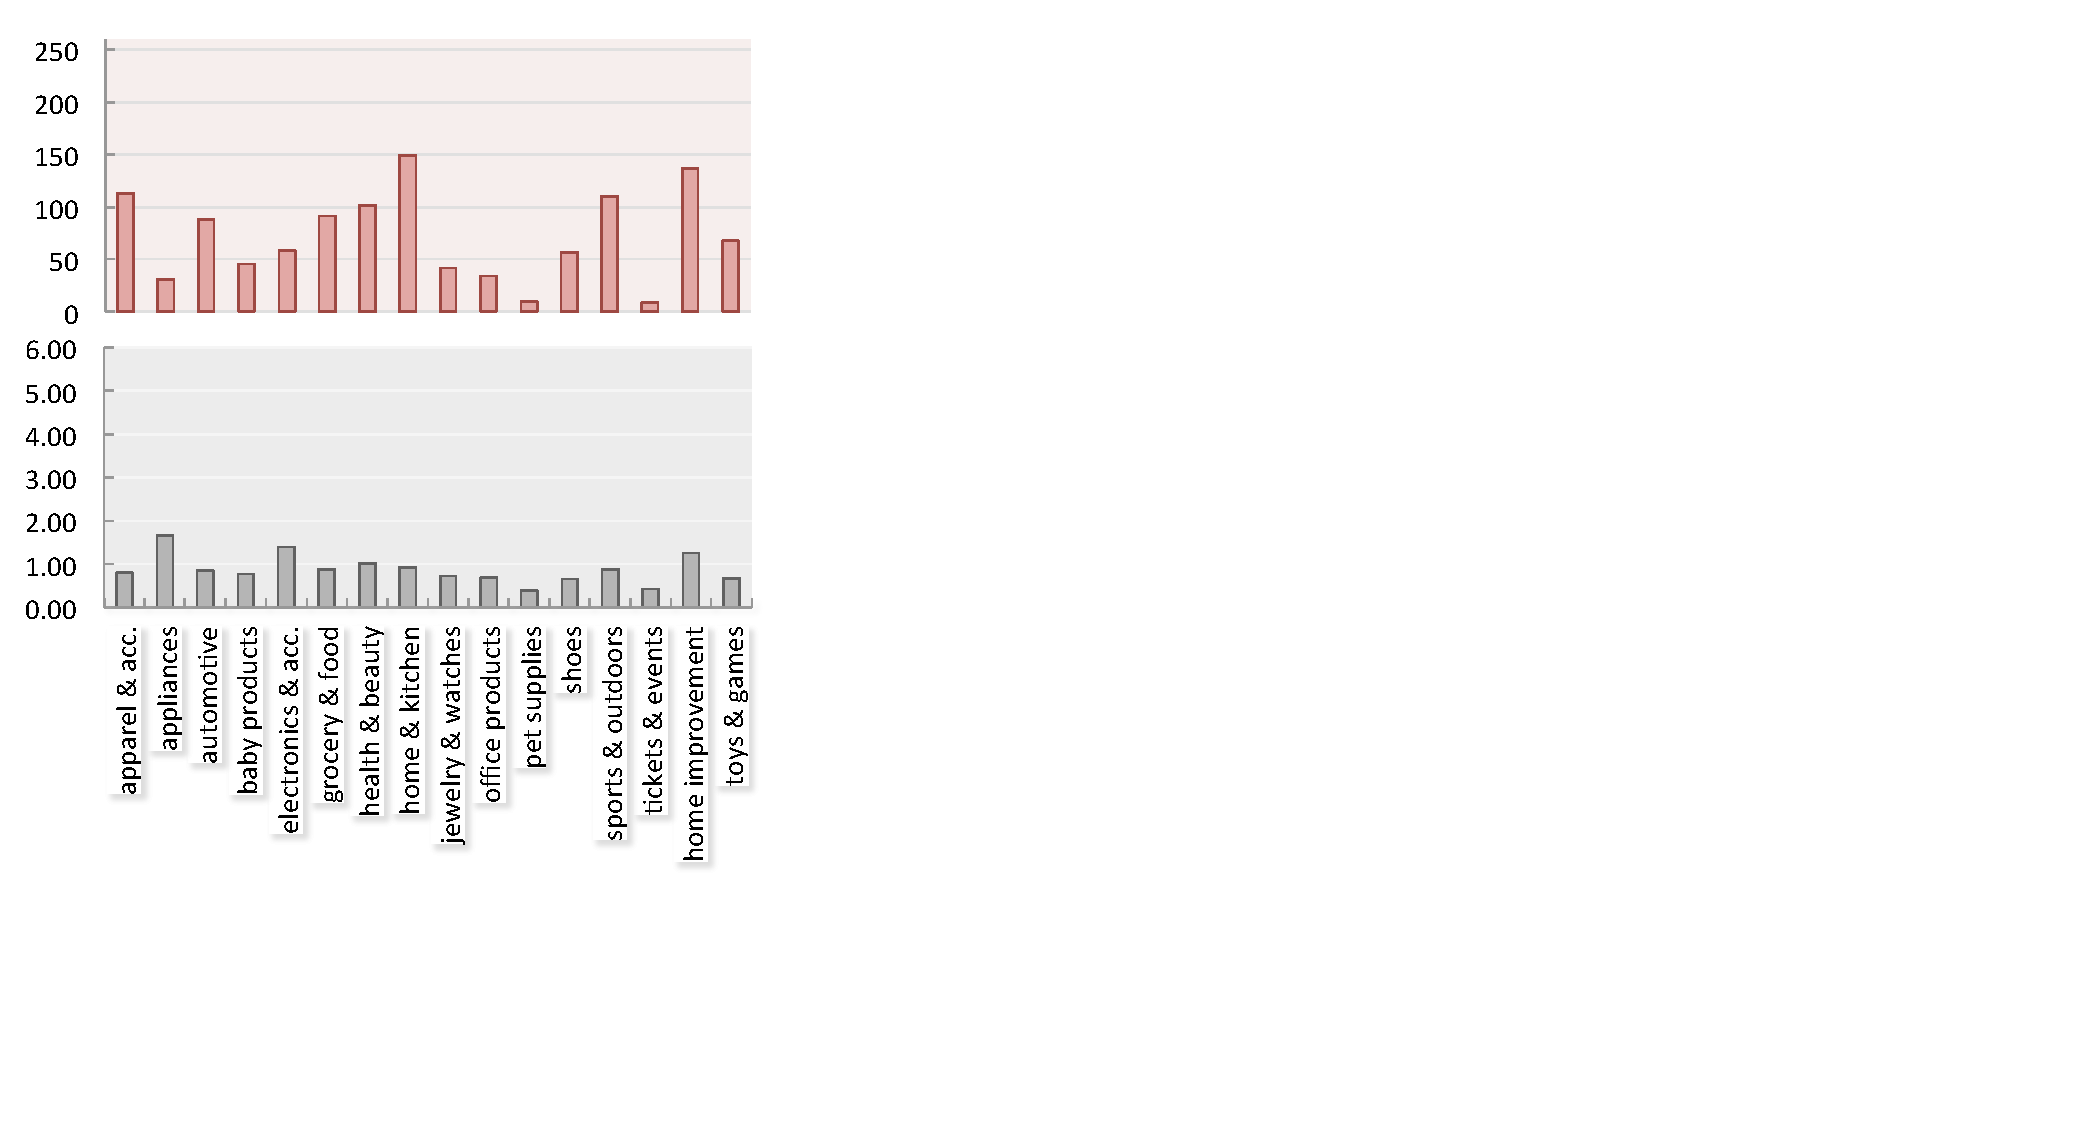
\includegraphics[width=0.3\textwidth]{images/BU1-branches+KL}} \hspace{0.1cm}
	\subfloat[{{\footnotesize AmazonJulian dataset: Total subtrees with taxonomy - 25; Total branches in all subtrees - 18188; Total listings in all subtrees - 7.46 million; Pearson correlation coeff. for branches vs. listings - 0.269. Top fig. vertical scale is 10x of Figs. \ref{Fig:BU1-branches+KL} and \ref{Fig:BU2-branches+KL} (top)}}]{\label{Fig:amazonj-branches+KL}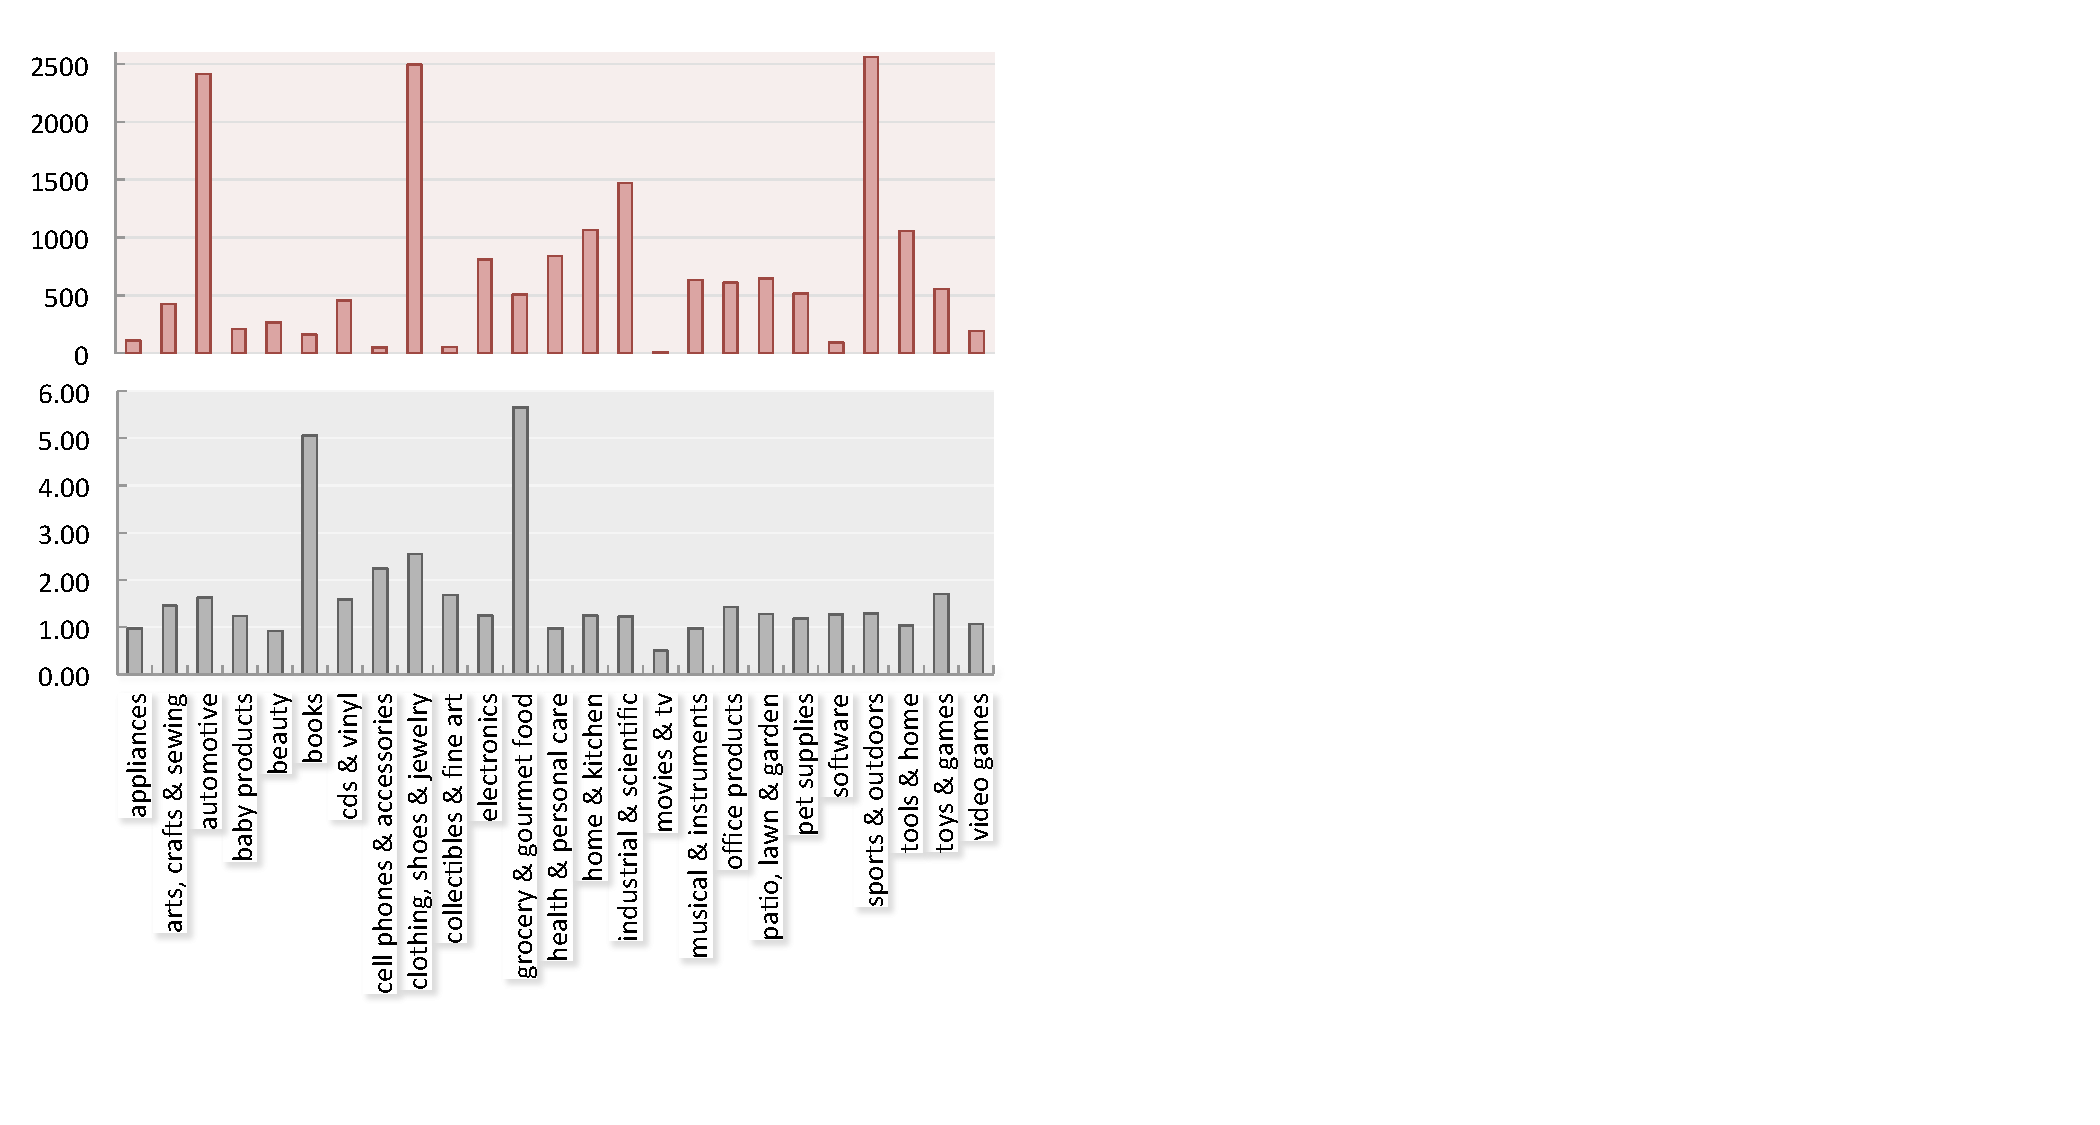
\includegraphics[width=0.35\textwidth]{images/AmazonJulian-branches+KL}} \hspace{0.1cm}
	\subfloat[{{\footnotesize BU2 dataset: Total subtrees with taxonomy - 15; Total branches in all subtrees - 571; Total listings in all subtrees - 60 million; Pearson correlation coeff. for branches vs. listings - 0.209}}]{\label{Fig:BU2-branches+KL}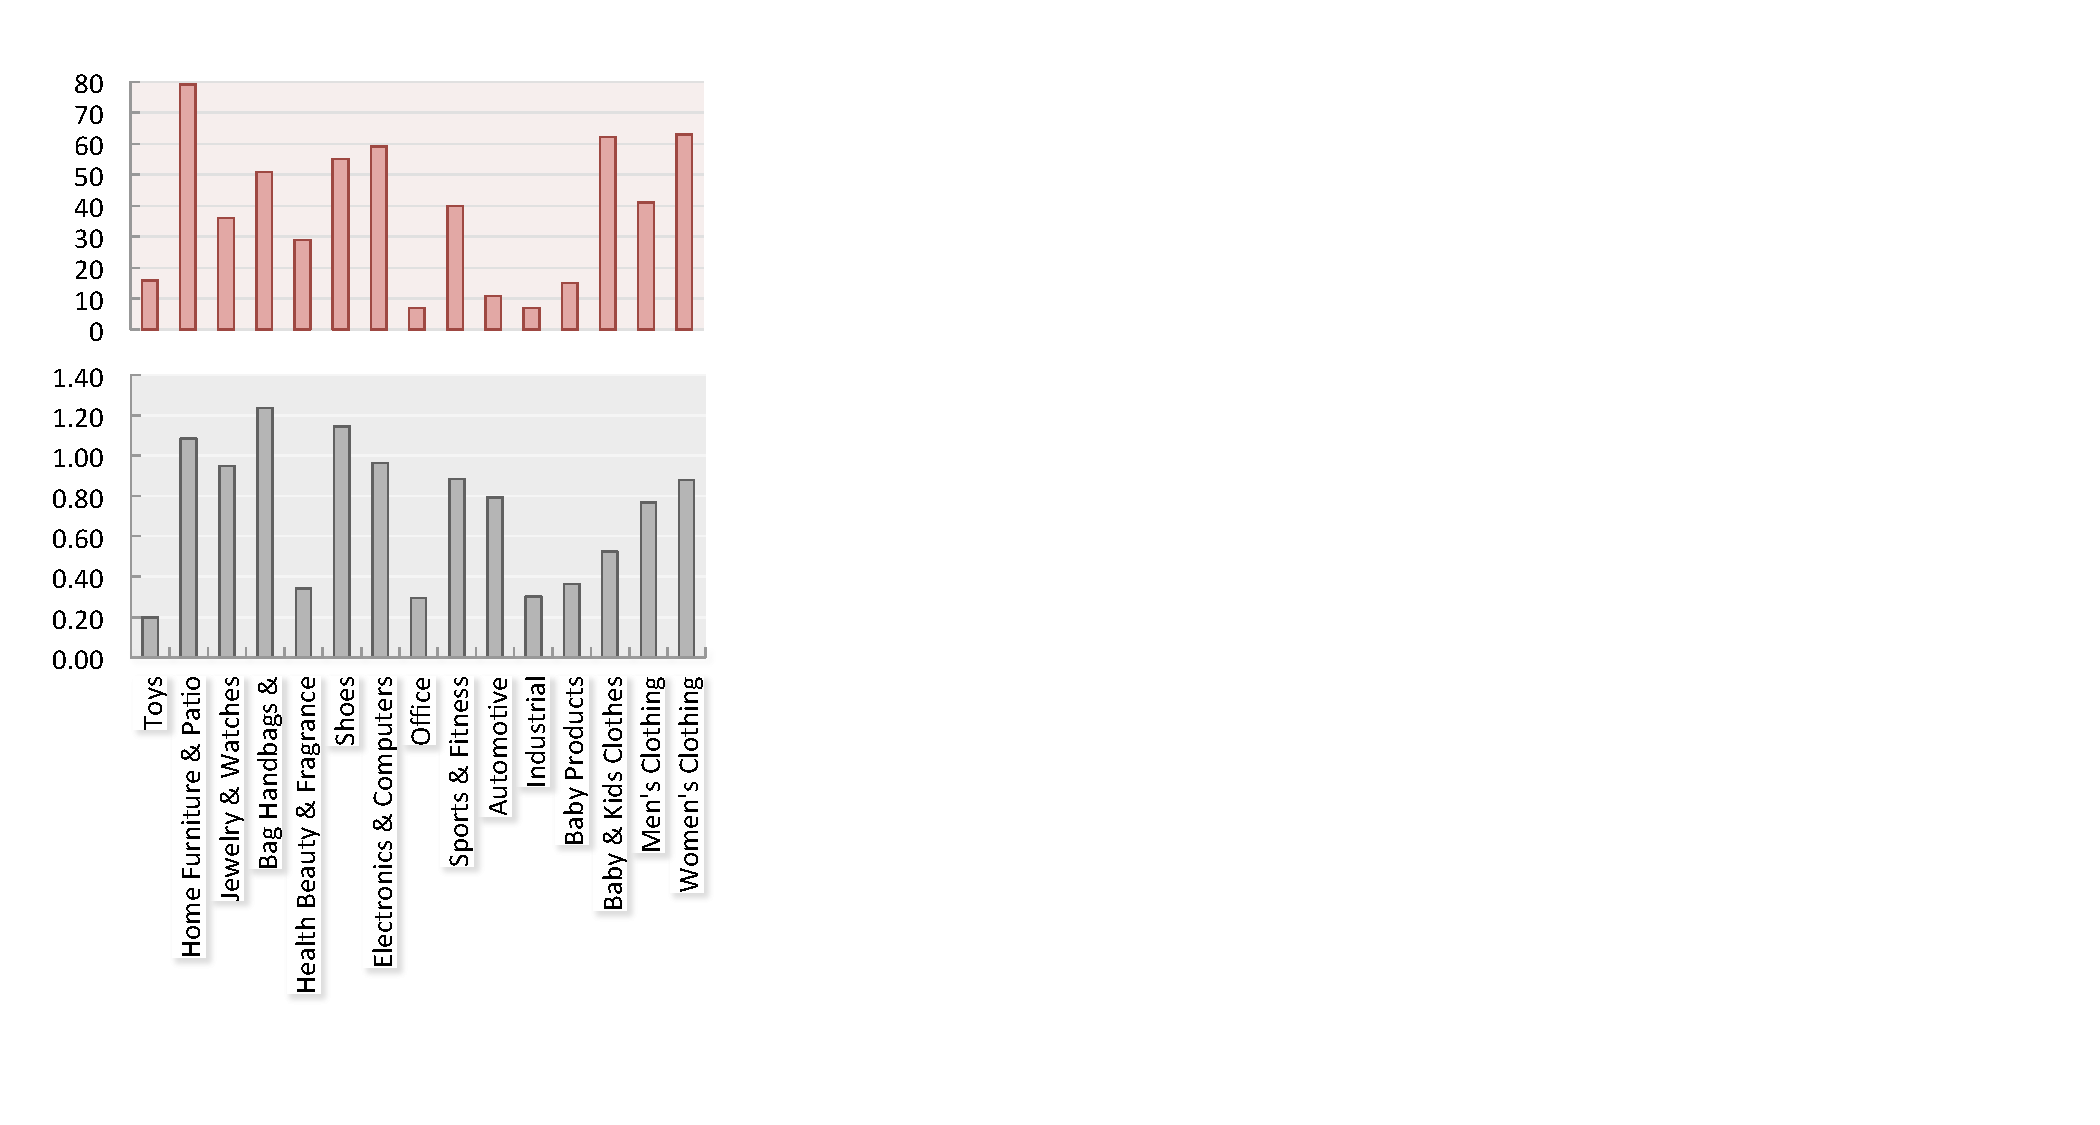
\includegraphics[width=0.27\textwidth]{images/BU2-branches+KL}}
	\vspace{-0.3cm}
	\caption{{\small Statistics on the datasets used for evaluation of classifiers: The top row shows the number of branches for a non-zero number of listings with titles for each dataset. The bottom row shows the KL divergence of the empirical distribution of listings in the branches in each subtree to the uniform distribution. These figures give us a rough measure of imbalance in each dataset. \textbf{The mean KL divergence values are: BU1 dataset - 0.872; AmazonJulian dataset - 1.654; BU2 dataset - 0.715}.}}
	\label{Fig:Dataset-statistics}
	\vspace{-0.6cm}
\end{figure}

An initial understanding of the imbalance in the datasets was important for us to judge expected generalization ability of several classifiers we experiment with. 
The top row in Fig. \ref{Fig:Dataset-statistics} shows the number of branches of level one taxonomy subtrees (i.e. class labels per level two category) for each of the datasets.
The AmazonJulian dataset (middle column) for taxonomy classification is the one obtained from \cite{Julian15}.
The dataset from BU1 (Fig. \ref{Fig:BU1-branches+KL}) shows the most \textit{benign} kind of imbalance with a Pearson correlation coefficient of the total number of listings to number of branches in each of the level one subtrees to be 0.643.
This means that the number of branches in the subtrees correlate well with the volume of listings.
The AmazonJulian dataset (henceforth AmazonJ) \cite{Julian15}, shows the highest number of branches in the subtrees on average.
This is possible since the extracted taxonomy may be a reflection of the navigational taxonomy which usually is listed in crawled product pages, instead of an internal data organization taxonomy.
An example is a branch named ``Clothing, Shoes \& Jewelry $\rightarrow$ G'' with many leaf nodes with names of brands starting with the letter 'G' such as ``G by GUESS'' to ``Gucci''.
However, for this dataset and that for BU2, the number of branches in the subtrees do not correlate well with the volume of listings indicating a much higher level of imbalance.

The bottom row of Fig. \ref{Fig:Dataset-statistics} shows the extra number of bits we would need to use to encode the listing distribution in the level one subtrees, if we thought the distribution was the uniform distribution i.e. balanced training set, but it was actually the empirical distribution emphasizing imbalance.
The mean of the KL divergence values in Fig. \ref{Fig:Dataset-statistics} hint towards the fact that, on average, classifiers that are more or less resistant to imbalance should perform about the same for BU1 and BU2 datasets but perform significantly worse for the AmazonJ dataset under identical feature transformations (see Section \ref{Subsect:results>imbalance-performance-expectations}).
